%----------------------------------------------------------------------------
%----------------------------------------------------------------------------
The collimated output of the three dye laser system is incident on a controlled sample of thermal molecular iodine. A circular aperture is placed immediately upstream from the sample to approximate a top hat spatial field in the interaction region. Initially, the sample is pure molecular iodine vapor at various concentrations - i.e., low buffer gas pressure. Once the various coherent processes of interest are verified (proof of concept), a buffer gas is introduced at various concentrations to measure the noise suppression limit of each of the coherent processes (efficiency).

The fluorescence signal from the interaction region is imaged onto the input slit of the monochromator by a lens system. The output of the monochromator may be read by either a CCD array (good for initial exploring and verification) or a PMT (temporally resolved and gated). The CCD image is directly downloaded into a PC for processing. The PMT signal is gated, amplified, and averaged (if necessary) in a gated boxcar averager system; the output of the boxcar system may then be read by either a chart recorder or a ADC equipped PC for processing. See figure \ref{block_fluorescence}.
%----------------------------------------------------------------------------
% block_fluorescence.tex
% by Troy Hix, May 2005
%----------------------------------------------------------------------------
\begin{figure}
\center
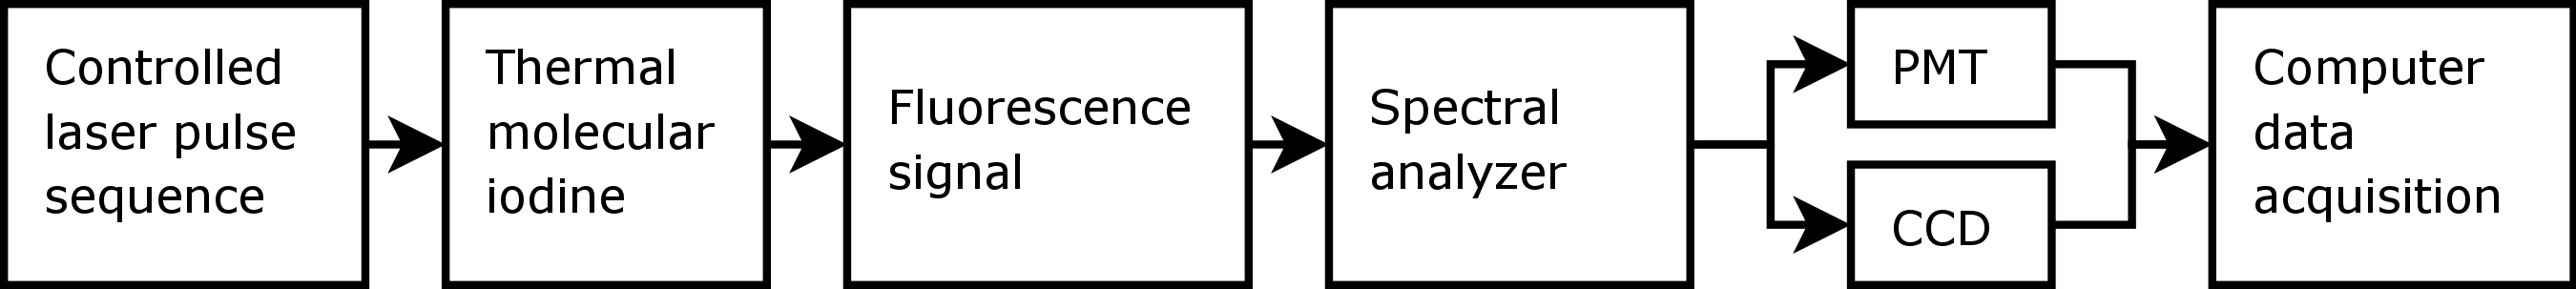
\includegraphics[width=6.00in]
{block_fluorescence/block_fluorescence.png}\\
\caption{Interaction and data acquisition block diagram}
\label{block_fluorescence}
\end{figure} 
%----------------------------------------------------------------------------
%----------------------------------------------------------------------------
%----------------------------------------------------------------------------



%----------------------------------------------------------------------------
%----------------------------------------------------------------------------
%----------------------------------------------------------------------------
%----------------------------------------------------------------------------
